%%% TeX-master: "../main.tex"
% kapitel5.tex
\chapter{Konkret getestete Applikationen}\label{chapter:concretetests}


Dieses Kapitel stellt nun einige Ergebnisse, die mittels des nach dem Konzepts tatsächlich
implementierten vollautomatischen GUI-Crawler und -Tester erzeugt wurden.
Als erstes getestetes Programm dient hierbei eine Enwicklerversion der von der
\textbf{e-Spirit AG} entwickelten Software \textbf{FirstSpirit} 
\footnote{\url{ http://www.e-spirit.com/de/produkt/arbeiten-mit-firstspirit/usability-fuer-redakteure/ }},
Version 5.2 DEV 201. Entwicklerversionen dieser Software enthalten zusätzliche,
dem normalen Nutzer unzugängliche Schaltflächen und Funktionen.


\section{Resultate FirstSpirit}\label{section:testresults}

Wie in den Graphdarstellungen auf Seiten \pageref{fig:model_firstspirit_notext} und 
\pageref{fig:model_freespirit_06.10.2015} zu sehen ist, enthält diese Version von
FirstSpirit etwa 34 einzigartige Fenster bzw. Zustände. Sie gehen fast alle vom
Hauptfenster des Programms bzw. dem Zustand zu Beginn des Tests aus,
nur einige wenige sind dahingegen tiefer abzweigend. Die Zahl einer im
Laufe eines vollen Durchgangs betätigter Eingabeelemente liegt im Vergleich bei
über 800. Dies legt nahe, dass umfangreiche interne Zustandsänderungen
möglich sind, die nicht direkt in von außen sichtbaren geänderten
Programmzuständen resultieren. Oder auch, dass eine Menge Eingabeelemente
existieren oder als solche erkannt wurden, deren Betätigung kein messbares
Resultat hatte.

Bedenkt man die Natur von FirstSpirit, ist dies keine große Überraschung.
FirstSpirit ist ein Content Management System bzw. CMS, im Grunde also
ein Client bzw. Editor für Webinhalte. Da der Autotester lediglich den Editor testet,
ohne Rücksicht auf die Inhalte nehmen zu wollen oder auch zu können,
hat die Mehrzahl der getätigten Eingaben keinen für das Konzept erkennbaren
Effekt. Änderungen am editierten Projekt haben aber für den Editor durchaus
-- wie auch immer geartete -- langfristige Konsequenzen, und es ist für
einen produktiven Einsatz des Autotesters anzuraten, solche von Seiteneffekten
beeinflussten Daten vor jedem Testdurchlauf wieder auf einen ursprünglichen
Zustand zurückzusetzen.

Nach Dutzenden von Testdurchläufen auf einem nie zurückgesetzten System
ist das von der e-Spirit AG genutzte Beispielprojekt \glqq{}Mithras\grqq{}
erheblich beschädigt. Zufällige Betätigung diverser Löschbefehle hat
Elemente aus dem Projekt entfernt bzw. Verknüpfungen gelöscht, die für
eine korrekte Funktion spezifischer Bestandteile nötig wären. Obwohl
dies natürlich Auswirkungen auf das Testverfahren hat, zeigt sich doch,
dass dennoch in etwa dieselbe Anzahl von Eingabeelementen getestet wird,
die graphische Oberfläche also nicht zwangsläufig auf ein korrekt funktionierendes
geladenes Projekt angewiesen ist, um alle möglichen Eingaben auszuprobieren.

In einer Produktivumgebung würde der Autotester folgendermaßen integriert:
Im Gegensatz zu Unit-Tests mit JUnit können keine festen Maßstäbe angelegt
werden, nach denen eine Version des Quellcodes zulässig ist oder auch nicht.
Korrektheit ist nicht das erklärte oder auch nur erreichbare Ziel.
Der Autotester wäre dementsprechend nicht im regulären automatischen
Build-Prozess enthalten (und diesen irgendwie anhalten oder behindern),
sondern wäre parallel angeordnet und kontinuierlich oder nach Wunsch
Tests durchführen. Man könnte sich z.B. vorstellen, dass eine neue
Programmversion jeweils fünfhundert (die Zahl ist völlig arbiträr) Durchläufe
des Autotesters auslöst und erfahren soll. Jede Instanz des Testprogramms wird
in einem virtualisiertem System gestartet, in das man vorher die
zentral gelagerte Konfigurationsdatei sowie die nötigen Voraussetzungen
kopiert hat -- in diesem Fall wäre dies das FirstSpirit-Programm sowie
die Dateien des Mithras-Projekts.

Die Logdateien und Ergebnis-Graphen jeder Instanz würden dann wieder zentral
gesammelt und könnten dann auf Gemeinsamkeiten und Abweichungen untersucht
werden. Instanzen, die nicht korrekt beendeten, sind natürlich von besonderem
Interesse. FirstSpirit hat eine eigene Schnittstelle, um Fehlerberichte von
aufgetretenen Ausnahmen weiterzureichen. Diese Berichte sowie in den Logdateien
erwähnte Fehlermeldungen könnten dann von Entwicklern genutzt werden, um
Schwachstellen im Code auszumerzen, wenn diese denn tatsächlich vorliegen.
Idealerweise ist es dem Autotester irgendwann unmöglich, Fehlermeldungen
oder Ausnahmen herbeizuführen, da die Entwickler jede ursprünglich 
unvorhergesehene Eingabe oder -sequenz abfangen oder korrekt behandeln.


\begin{sidewaysfigure}
	\centering
	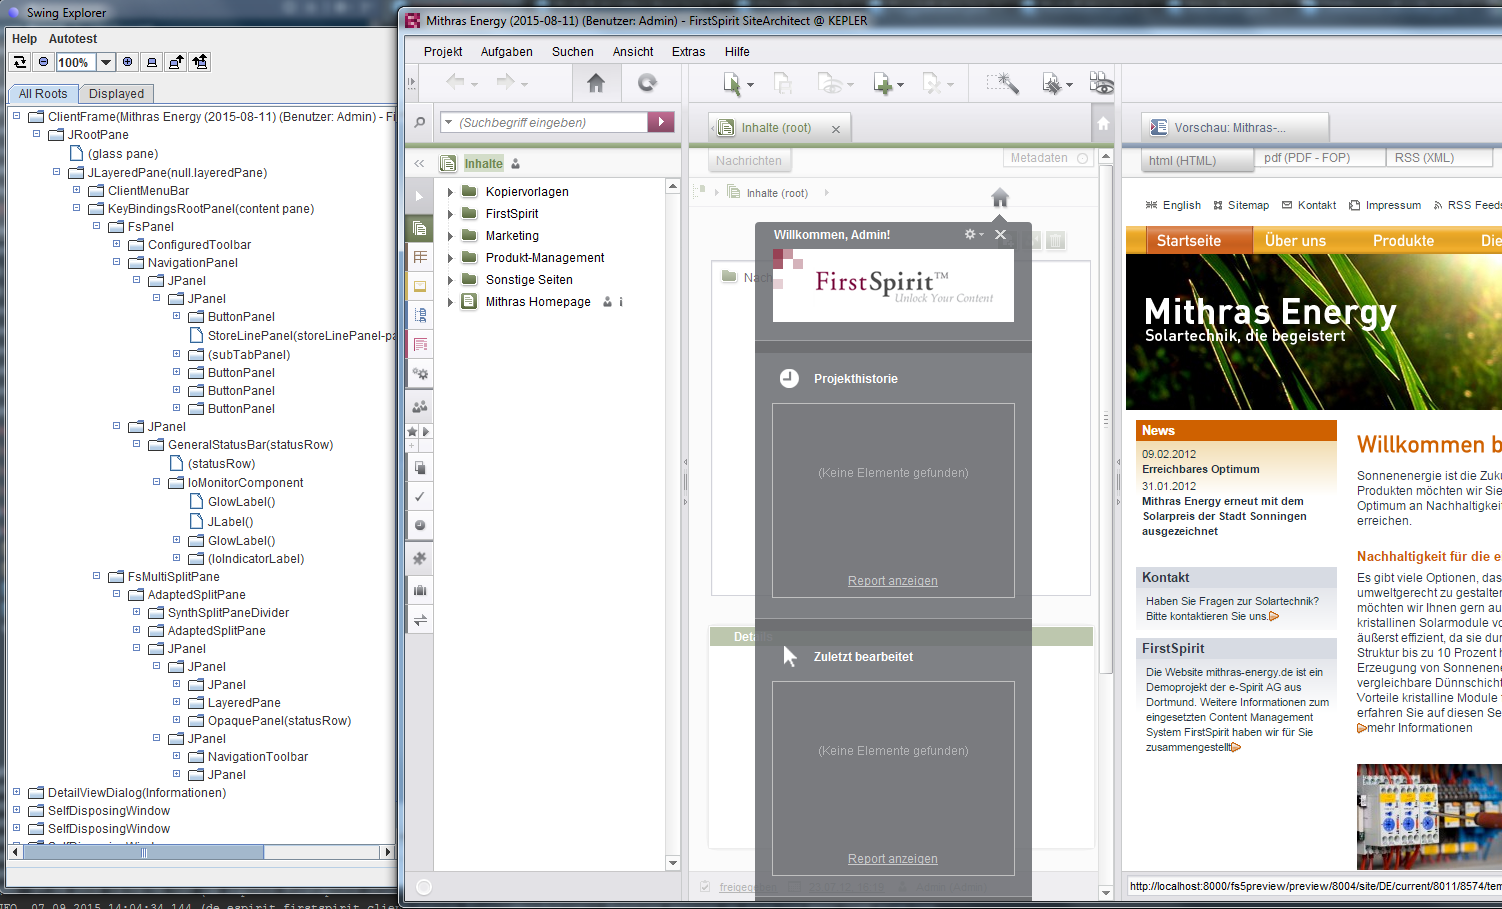
\includegraphics[width=0.85\textwidth]{bilder/screenshot_freespirit.png}
	\caption{Screenshot der e-Spirit CMS-Anwendung FirstSpirit
	sowie anhängigem Swing Explorer, der den Komponentenbaum der Applikation darstellt}
	\label{fig:screenshot_freespirit}
\end{sidewaysfigure}

\begin{figure}
	\centering
	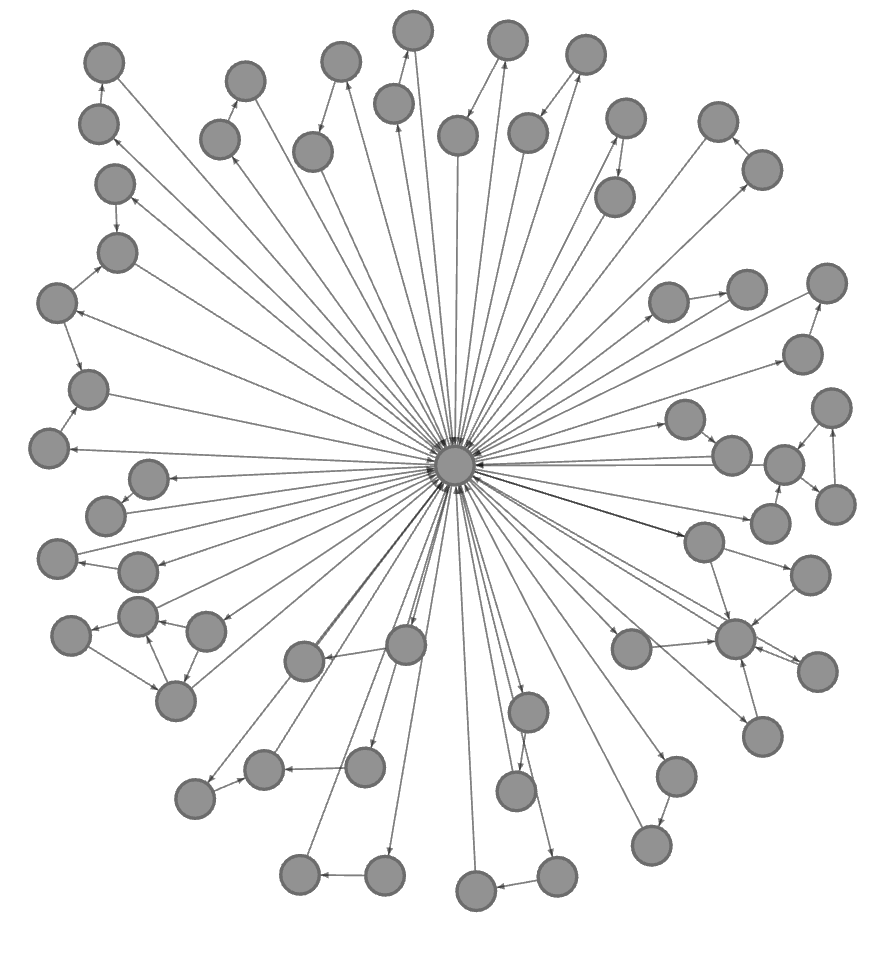
\includegraphics[width=0.85\textwidth]{bilder/model_firstspirit_notext.png}
	\caption{mit Gephi und dem Yifan Hu Algorithmus \cite{hu2005efficient}
    sowie noch für Lesbarkeit maneull angepasste visualierte Graphausgabe 
	des Autotesters über FirstSpirit, hoher Zoomfaktor, keine Beschriftungen.
	Die Pfeile des gerichteten Graphen sind so sichtbar.}
	\label{fig:model_firstspirit_notext}
\end{figure}

\begin{sidewaysfigure}
	\centering
	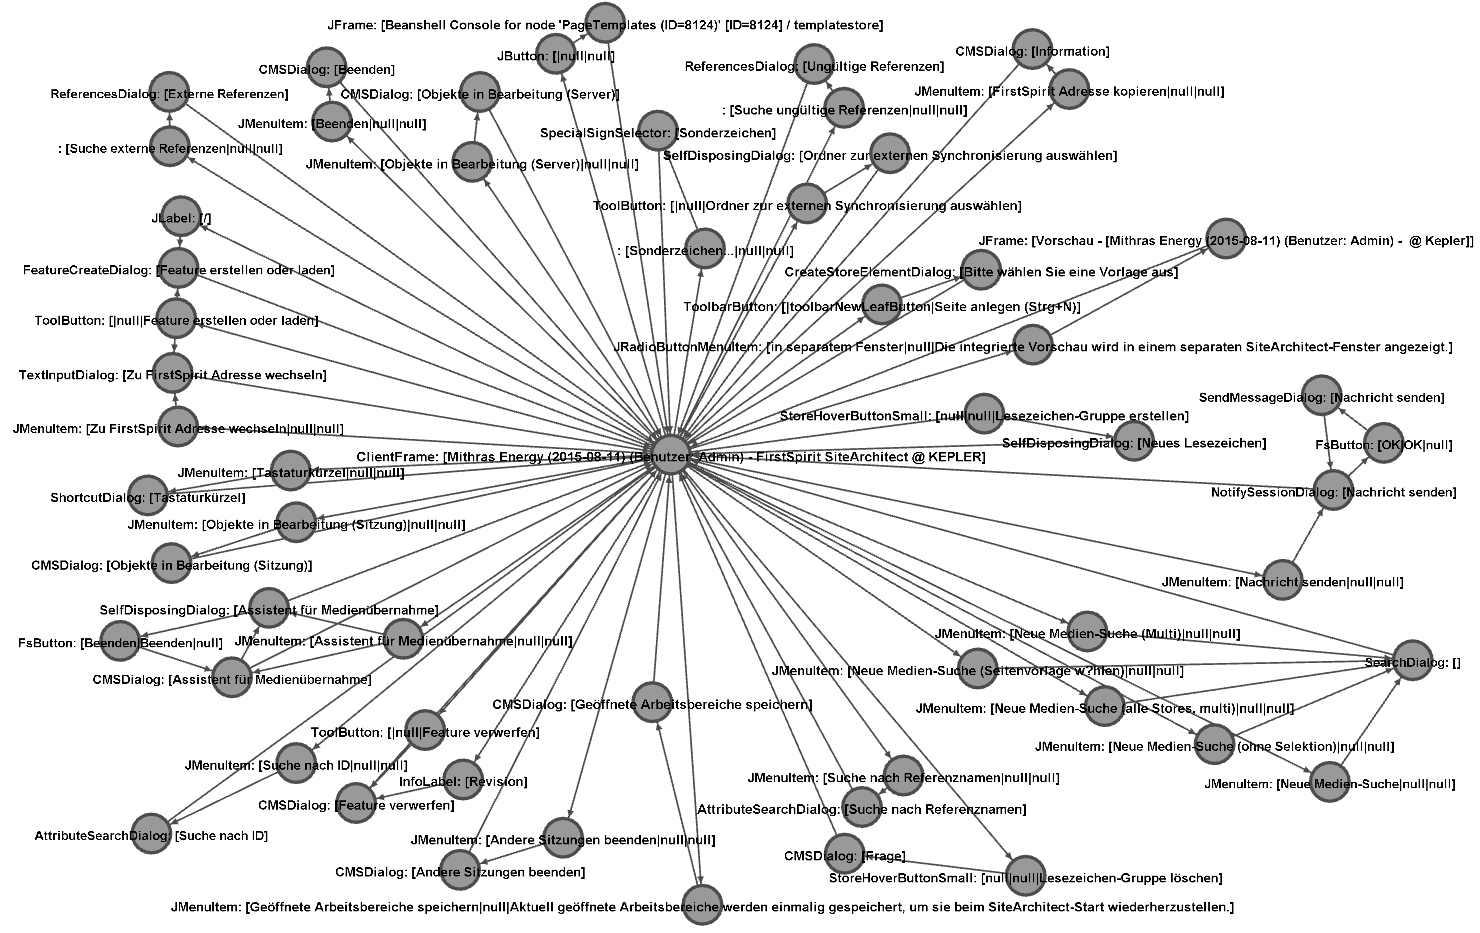
\includegraphics[width=0.85\textwidth]{bilder/model_freespirit.png}
	\caption{mit Gephi und dem Yifan Hu Algorithmus \cite{hu2005efficient}
    sowie noch für Lesbarkeit maneull angepasste visualierte Graphausgabe 
	des Autotesters über FirstSpirit bei einem der ergiebigeren Durchläufe.
	Beschriftungen der Knoten sind deaktiviert.}
	\label{fig:model_freespirit_06.10.2015}
\end{sidewaysfigure}



Die Knoten sind in Dreiergruppen angeordnet: Ein Ursprungsfenster, ein Übergangsknoten
(bzw. ein Wort des Modells), sowie der resultierende Zustand bzw. das sich öffnende Fenster.
Dies ist schlicht eine Frage der Lesbarkeit -- anstelle der mittleren Knoten für Übergänge sollten
eigentlich einfach beschriftete Kanten benutzt werden, aber dies schränkt die Möglichkeiten,
den anhängigen Text in eine lesbare Form zu bringen, zu stark ein. Es ist schlicht zu viel
Textinformation, um mit einer Legende o.Ä. auszukommen.


\section{Vergleich mit klassischen Tests}\label{section:testcomparisonclassic}

Ein Vergleich mit halbautomatischen Methoden oder gewöhnlichen Unit-Tests
ist erst einmal schwierig, da diese auf anderen Prinzipien aufbauen.
Üblicherweise ist das Ziel die Überprüfung der Korrektheit des Programms.
Um eine Aussage über Korrektheit treffen zu können, sind kontextuelle
Informationen über ein Programm bzw. das gewünschte Verhalten notwendig.
Einem vollautomatischen Ansatz stehen diese Informationen schlicht nicht
zur Verfügung. Das hier vorgestellte Konzept ist auch nicht als Ersatz 
klassischer Tests gedacht oder in irgendeiner Form äquivalent.

Getreu dem Zitat von Dijkstra \footnote{ACM Turing Lecture 1972},
nach dem die Abwesenheit von Fehlern nicht bewiesen werden kann,
zielt der Autotester in eine andere Richtung. Es wird versucht, so viele
unerwartete Situationen und resultierende Fehler zu erzeugen, wie
irgendwie möglich. Man kann ihn also als ein Komplement bzw. eine Addition
zu klassischen Tests verstehen bzw. Einsetzen.

Ein Durchlauf des Autotesters ist verglichen mit Unit Tests und den
meisten Regressionstests sehr langsam. Ein vollständiger Durchlauf
über FirstSpirit dauert ungefähr 20 Minuten. Leider gibt es für die
Emulation menschlicher Eingaben und der Wartezeit für die Verarbeitung
dieser Eingaben durch das Programm keine guten Alternativen.
Man bedenke allerdings: Derselbe Test durch einen Menschen würde
noch erheblich länger dauern und die üblichen menschlichen Fehlerquellen
beinhalten, die das Ergebnis zusätzlich beeinflussen.
